\section{PostgreSQL Internals}

%%%%%%%%%%%%%%%%%%%%%%%%%%%%%%%%%%%%%%%%%%%%%%%%%%%%%%%%%%%%%%%%%%%%%%%%%%%%%%%%

\subsection{Point in Time Recovery}

%%%%%%%%%%%%%%%%%%%%%%%%%%%%%%%%%%%%%%%%%%%%%%%%%%%%%%%%%%%%%%%%%%%%%%%%%%%%%%%%

\begin{frame}{Cycle des données dans PostgreSQL}

\begin{figure}
\begin{center}
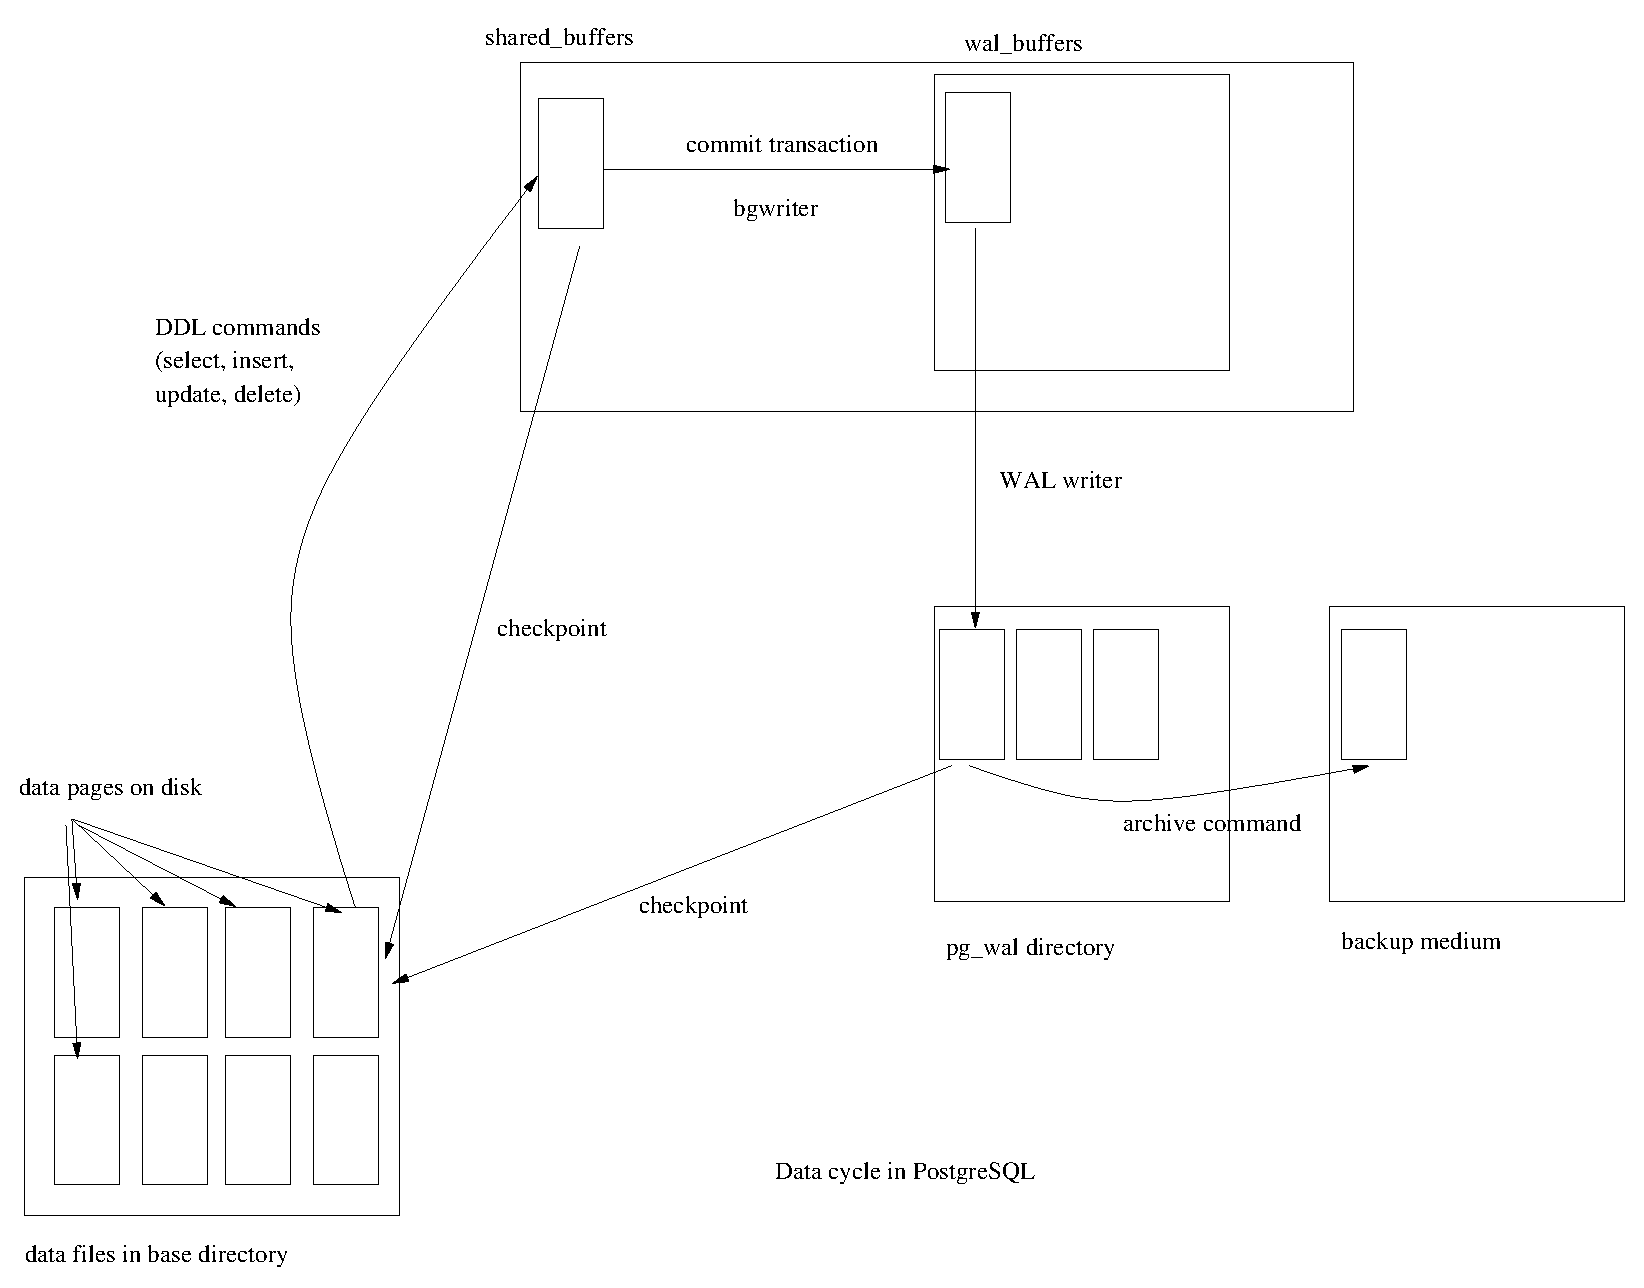
\includegraphics[angle=0, width=0.5\textwidth]{images/internals.eps}
\end{center}
\end{figure}

\begin{toile}
\toileurl{https://www.postgresql.org/docs/15/wal-configuration.html}
\end{toile}

\end{frame}

%%%%%%%%%%%%%%%%%%%%%%%%%%%%%%%%%%%%%%%%%%%%%%%%%%%%%%%%%%%%%%%%%%%%%%%%%%%%%%%%

\begin{frame}{L'importance des sauvegardes}

\begin{itemize}

\item Il est important de posséder 2 copies supplémentaires à la copie des données de productions.
\item Une des 2 copies se situe hors site.
\item Chacune des 2 copies est stockée sur un média différent.

\end{itemize}

\begin{toile}
\toileurl{https://www.it-connect.fr/sauvegarde-quest-ce-que-la-regle-du-3-2-1/}
\end{toile}

\end{frame}

%%%%%%%%%%%%%%%%%%%%%%%%%%%%%%%%%%%%%%%%%%%%%%%%%%%%%%%%%%%%%%%%%%%%%%%%%%%%%%%%

\begin{frame}[fragile]{Différents types de sauvegardes}

Il existe différents types de sauvegarde:

\begin{itemize}

   \item logique avec les commandes \commande{pg\_dump} et \commande{pg\_dumpall}
   \item au niveau du système de fichiers avec la commande \commande{tar}.\footnote{La sauvegarde du système de fichiers n'est pas recommandée par la documentation officielle de PostgreSQL}
   \item binaire avec la commande \commande{pg\_basebackup}

\end{itemize}

\begin{toile}
\toileurl{https://www.postgresql.org/docs/15/backup.html}
\end{toile}

\end{frame}

%%%%%%%%%%%%%%%%%%%%%%%%%%%%%%%%%%%%%%%%%%%%%%%%%%%%%%%%%%%%%%%%%%%%%%%%%%%%%%%%

\begin{frame}[fragile]{Mise en place de la génération des WAL (1/2)}

\begin{itemize}

   \item Pour activer la génération des WAL, merci de modifier les paramètres suivants dans \textit{postgresql.conf}

\begin{intercom}
wal\_level = replica # or higher
archive\_mode = on
[...]
\end{intercom}

\end{itemize}

\begin{toile}
\toileurl{https://www.postgresql.org/docs/15/continuous-archiving.html}
\end{toile}

\end{frame}

%%%%%%%%%%%%%%%%%%%%%%%%%%%%%%%%%%%%%%%%%%%%%%%%%%%%%%%%%%%%%%%%%%%%%%%%%%%%%%%%

\begin{frame}[fragile]{\commande{archive\_command} et \commande{archive\_library}}

\begin{itemize}

   \item La copie des WAL vers le système de sauvegarde se paramètre depuis les 2 valeurs suivantes:

   \begin{itemize}
      \item \textbf{archive\_command}: Commandes shell d'archivage des WAL
      \item \textbf{archive\_library}: Binaire d'archivage des WAL
   \end{itemize}

   \item Chacune des 2 valeur s'utilise au choix. Elles ne peuvent utilisées en même temps.
   \item Pour les exercices, le paramètre \textbf{archive\_command} sera utilisé.

\begin{scriptsize}
   \begin{intercom}
archive\_command = 'test ! -f /mnt/server/archivedir/\%f && cp \%p /mnt/server/archivedir/\%f' # Unix
   [...]
   \end{intercom}
\end{scriptsize}

\end{itemize}

\end{frame}

%%%%%%%%%%%%%%%%%%%%%%%%%%%%%%%%%%%%%%%%%%%%%%%%%%%%%%%%%%%%%%%%%%%%%%%%%%%%%%%%

\begin{frame}[fragile]{Fonctionnement de l'archivage des WAL}

\begin{itemize}

   \item La commande d'archivage des WALs est lancée par le même utilisateur du process \textit{postmaster}
   \item Elle est censée renvoyer un code différent de 0 en cas d'erreur
   \item Il est important de vérifier que le WAL n'existe pas dans le répertoire cible sous peine de l'écraser
   \item En cas d'erreur d'archivage, PostgreSQL retente autant de fois que nécessaire
   \item Tant que le fichier WAL n'est pas archivé, celui-ci n'est pas supprimé du répertoire pg\_wal, ce qui peut amener à une saturation du système de fichiers
   \item En cas de saturation du répertoire pg\_wal, le serveur s'arrête avec une erreur de type PANIC. Il pourra redémarrer une fois qu'il aura de l'espace disque disponible

\end{itemize}

\end{frame}

%%%%%%%%%%%%%%%%%%%%%%%%%%%%%%%%%%%%%%%%%%%%%%%%%%%%%%%%%%%%%%%%%%%%%%%%%%%%%%%%

\begin{frame}[fragile]{Caractéristique des WAL}

\begin{itemize}

   \item Le nom des fichiers WAL inclut jusqu'à 64 caractères
   \item Il est composé de lettres ASCII, de chiffres et de points
   \item Il est important de garder le nom de l'archive WAL
   \item La sauvegarde des WALs ne permet pas de restaurer \textit{postgresql.conf}, \textit{pg\_hba.conf} ou \textit{pg\_ident.conf}
   \item Il est important de sauvegarder ces 3 fichiers indépendamment
   \item Ces fichiers peuvent être stockés dans un répertoire paramétrable

\end{itemize}

\end{frame}

%%%%%%%%%%%%%%%%%%%%%%%%%%%%%%%%%%%%%%%%%%%%%%%%%%%%%%%%%%%%%%%%%%%%%%%%%%%%%%%%

\begin{frame}[fragile]{La commande \commande{pg\_basebackup}}

\begin{itemize}

\item La commande \commande{pg\_basebackup} sauvegarde un cluster PostgreSQL
\item Elle ne s'applique sur une base de données en particulier
\item L'utilisateur lançant cette commande doit posséder le droit \textbf{REPLICATION} ou être un super-utilisateur
\item La commande peut être lancée sur un serveur standby
\item La table \textit{pg\_stat\_progress\_basebackup} donne une idée de la progression de la commande

\end{itemize}

\begin{toile}
\toileurl{https://www.postgresql.org/docs/15/app-pgbasebackup.html}
\toileurl{https://www.postgresql.org/docs/15/progress-reporting.html\#BASEBACKUP-PROGRESS-REPORTING}
\end{toile}

\end{frame}

%%%%%%%%%%%%%%%%%%%%%%%%%%%%%%%%%%%%%%%%%%%%%%%%%%%%%%%%%%%%%%%%%%%%%%%%%%%%%%%%

\begin{frame}{\path{/dev}}

\begin{itemize}

\item Le pseudo-système de fichiers \path{/dev} contient les fichiers spéciaux
permettant l'accès au matériel.

\item Ces fichiers spéciaux sont adaptés au matériel détecté par le noyau lors
de son démarrage et les fichiers idoines sont créés ou supprimés dynamiquement
par la suite en fonction du branchement ou du débranchement de périphériques.

\item C'est un système nommé « udev », dont le fonctionnement est réparti entre
le noyau et un daemon, qui gère le pseudo-système de fichiers \path{/dev}. Il
est au programme de l'examen 201.

\end{itemize}

\begin{toile}
\toileurl{http://fr.wikipedia.org/wiki/Udev}
\end{toile}

\end{frame}

%%%%%%%%%%%%%%%%%%%%%%%%%%%%%%%%%%%%%%%%%%%%%%%%%%%%%%%%%%%%%%%%%%%%%%%%%%%%%%%%

\newlength{\largeurtableau}
\setlength{\largeurtableau}{\textwidth}
\addtolength{\largeurtableau}{-2\leftmarginii}

%%%%%%%%%%%%%%%%%%%%%%%%%%%%%%%%%%%%%%%%%%%%%%%%%%%%%%%%%%%%%%%%%%%%%%%%%%%%%%%%

\begin{frame}{\path{/proc}}

\begin{itemize}

\item Le pseudo-système de fichiers \path{/proc} contient :

	\begin{itemize}

	\item un répertoire par processus, nommé selon son PID

	\item un lien symbolique \path{self} pointant vers le répertoire
	correspondant au processus courant

	\item divers fichiers contenant des informations générales, par
	exemple :

\bigskip

\begin{tabulary}{\largeurtableau}{lJ}
\hline
\path{/proc/cmdline}	& paramètres passés au noyau par le chargeur
				d'amorçage		\\
\path{/proc/cpuinfo}	& microprocesseur(s)		\\
\path{/proc/interrupts}	& interruptions			\\
\path{/proc/loadavg}	& charge moyenne		\\
\path{/proc/meminfo}	& utilisation de la mémoire	\\
\hline
\end{tabulary}

	\end{itemize}

\end{itemize}

\begin{toile}
\toileurl{http://fr.wikipedia.org/wiki/Procfs}
\end{toile}

\end{frame}

%%%%%%%%%%%%%%%%%%%%%%%%%%%%%%%%%%%%%%%%%%%%%%%%%%%%%%%%%%%%%%%%%%%%%%%%%%%%%%%%

\begin{frame}[fragile]{\path{/sys}}

\begin{itemize}

\item Le pseudo-système de fichiers \path{/sys} fournit de nombreuses
informations concernant le matériel et les pilotes.

\item Exemple :

\begin{intercom}
\$ cat /sys/class/net/eth0/address
00:1c:23:30:20:13
\end{intercom}

\end{itemize}

\begin{toile}
\toileurl{http://fr.wikipedia.org/wiki/Sysfs}
\end{toile}

\end{frame}

%%%%%%%%%%%%%%%%%%%%%%%%%%%%%%%%%%%%%%%%%%%%%%%%%%%%%%%%%%%%%%%%%%%%%%%%%%%%%%%%

\subsection{Démarrage du système}

%%%%%%%%%%%%%%%%%%%%%%%%%%%%%%%%%%%%%%%%%%%%%%%%%%%%%%%%%%%%%%%%%%%%%%%%%%%%%%%%

% TODO démarrage single user

%%%%%%%%%%%%%%%%%%%%%%%%%%%%%%%%%%%%%%%%%%%%%%%%%%%%%%%%%%%%%%%%%%%%%%%%%%%%%%%%

% TODO Provide common commands to the boot loader and options to the kernel at boot time.
% TODO Demonstrate knowledge of the boot sequence from BIOS to boot completion.
% TODO Check boot events in the log files.

% TODO /var/log/messages

%%%%%%%%%%%%%%%%%%%%%%%%%%%%%%%%%%%%%%%%%%%%%%%%%%%%%%%%%%%%%%%%%%%%%%%%%%%%%%%%

\subsection{Changement de niveaux d'exécution et arrêt ou redémarrage du système}

%%%%%%%%%%%%%%%%%%%%%%%%%%%%%%%%%%%%%%%%%%%%%%%%%%%%%%%%%%%%%%%%%%%%%%%%%%%%%%%%

\begin{frame}{Les commandes \commande{halt}, \commande{poweroff} et
\commande{reboot}}

\begin{itemize}

\item Équivalentes à la commande \commande{shutdown} utilisée avec certaines
options :

\bigskip

\begin{tabular}{|l|l|}
\hline
\commande{halt}		& \commande{shutdown} \option{-H}	\\
\hline
\commande{poweroff}	& \commande{shutdown} \option{-P}	\\
\hline
\commande{reboot}	& \commande{shutdown} \option{-r}	\\
\hline
\end{tabular}

\bigskip

\item Contrairement à \commande{shutdown}, ces commandes ne permettent
d'indiquer ni de délai (elles ont un effet immédiat) ni de message pour les
utilisateurs connectés.

\end{itemize}

\begin{toile}
\toileurl{http://fr.wikipedia.org/wiki/Halt}
\end{toile}

\end{frame}

%%%%%%%%%%%%%%%%%%%%%%%%%%%%%%%%%%%%%%%%%%%%%%%%%%%%%%%%%%%%%%%%%%%%%%%%%%%%%%%%

% TODO Knowledge of basic features of systemd and Upstart.
